\documentclass[1p]{elsarticle_modified}
%\bibliographystyle{elsarticle-num}

%\usepackage[colorlinks]{hyperref}
%\usepackage{abbrmath_seonhwa} %\Abb, \Ascr, \Acal ,\Abf, \Afrak
\usepackage{amsfonts}
\usepackage{amssymb}
\usepackage{amsmath}
\usepackage{amsthm}
\usepackage{scalefnt}
\usepackage{amsbsy}
\usepackage{kotex}
\usepackage{caption}
\usepackage{subfig}
\usepackage{color}
\usepackage{graphicx}
\usepackage{xcolor} %% white, black, red, green, blue, cyan, magenta, yellow
\usepackage{float}
\usepackage{setspace}
\usepackage{hyperref}

\usepackage{tikz}
\usetikzlibrary{arrows}

\usepackage{multirow}
\usepackage{array} % fixed length table
\usepackage{hhline}

%%%%%%%%%%%%%%%%%%%%%
\makeatletter
\renewcommand*\env@matrix[1][\arraystretch]{%
	\edef\arraystretch{#1}%
	\hskip -\arraycolsep
	\let\@ifnextchar\new@ifnextchar
	\array{*\c@MaxMatrixCols c}}
\makeatother %https://tex.stackexchange.com/questions/14071/how-can-i-increase-the-line-spacing-in-a-matrix
%%%%%%%%%%%%%%%

\usepackage[normalem]{ulem}

\newcommand{\msout}[1]{\ifmmode\text{\sout{\ensuremath{#1}}}\else\sout{#1}\fi}
%SOURCE: \msout is \stkout macro in https://tex.stackexchange.com/questions/20609/strikeout-in-math-mode

\newcommand{\cancel}[1]{
	\ifmmode
	{\color{red}\msout{#1}}
	\else
	{\color{red}\sout{#1}}
	\fi
}

\newcommand{\add}[1]{
	{\color{blue}\uwave{#1}}
}

\newcommand{\replace}[2]{
	\ifmmode
	{\color{red}\msout{#1}}{\color{blue}\uwave{#2}}
	\else
	{\color{red}\sout{#1}}{\color{blue}\uwave{#2}}
	\fi
}

\newcommand{\Sol}{\mathcal{S}} %segment
\newcommand{\D}{D} %diagram
\newcommand{\A}{\mathcal{A}} %arc


%%%%%%%%%%%%%%%%%%%%%%%%%%%%%5 test

\def\sl{\operatorname{\textup{SL}}(2,\Cbb)}
\def\psl{\operatorname{\textup{PSL}}(2,\Cbb)}
\def\quan{\mkern 1mu \triangleright \mkern 1mu}

\theoremstyle{definition}
\newtheorem{thm}{Theorem}[section]
\newtheorem{prop}[thm]{Proposition}
\newtheorem{lem}[thm]{Lemma}
\newtheorem{ques}[thm]{Question}
\newtheorem{cor}[thm]{Corollary}
\newtheorem{defn}[thm]{Definition}
\newtheorem{exam}[thm]{Example}
\newtheorem{rmk}[thm]{Remark}
\newtheorem{alg}[thm]{Algorithm}

\newcommand{\I}{\sqrt{-1}}
\begin{document}

%\begin{frontmatter}
%
%\title{Boundary parabolic representations of knots up to 8 crossings}
%
%%% Group authors per affiliation:
%\author{Yunhi Cho} 
%\address{Department of Mathematics, University of Seoul, Seoul, Korea}
%\ead{yhcho@uos.ac.kr}
%
%
%\author{Seonhwa Kim} %\fnref{s_kim}}
%\address{Center for Geometry and Physics, Institute for Basic Science, Pohang, 37673, Korea}
%\ead{ryeona17@ibs.re.kr}
%
%\author{Hyuk Kim}
%\address{Department of Mathematical Sciences, Seoul National University, Seoul 08826, Korea}
%\ead{hyukkim@snu.ac.kr}
%
%\author{Seokbeom Yoon}
%\address{Department of Mathematical Sciences, Seoul National University, Seoul, 08826,  Korea}
%\ead{sbyoon15@snu.ac.kr}
%
%\begin{abstract}
%We find all boundary parabolic representation of knots up to 8 crossings.
%
%\end{abstract}
%\begin{keyword}
%    \MSC[2010] 57M25 
%\end{keyword}
%
%\end{frontmatter}

%\linenumbers
%\tableofcontents
%
\newcommand\colored[1]{\textcolor{white}{\rule[-0.35ex]{0.8em}{1.4ex}}\kern-0.8em\color{red} #1}%
%\newcommand\colored[1]{\textcolor{white}{ #1}\kern-2.17ex	\textcolor{white}{ #1}\kern-1.81ex	\textcolor{white}{ #1}\kern-2.15ex\color{red}#1	}

{\Large $\underline{12a_{0345}~(K12a_{0345})}$}

\setlength{\tabcolsep}{10pt}
\renewcommand{\arraystretch}{1.6}
\vspace{1cm}\begin{tabular}{m{100pt}>{\centering\arraybackslash}m{274pt}}
\multirow{5}{120pt}{
	\centering
	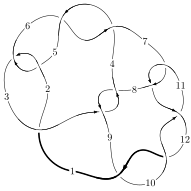
\includegraphics[width=112pt]{../../../GIT/diagram.site/Diagrams/png/1146_12a_0345.png}\\
\ \ \ A knot diagram\footnotemark}&
\allowdisplaybreaks
\textbf{Linearized knot diagam} \\
\cline{2-2}
 &
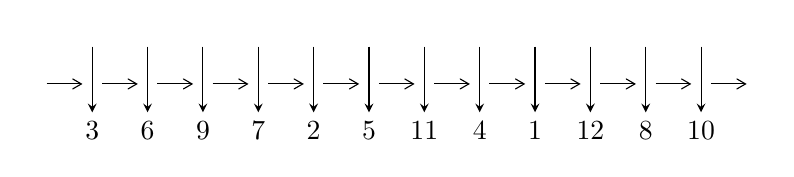
\begin{tikzpicture}[x=20pt, y=17pt]
	% nodes
	\node (C0) at (0, 0) {};
	\node (C1) at (1, 0) {};
	\node (C1U) at (1, +1) {};
	\node (C1D) at (1, -1) {3};

	\node (C2) at (2, 0) {};
	\node (C2U) at (2, +1) {};
	\node (C2D) at (2, -1) {6};

	\node (C3) at (3, 0) {};
	\node (C3U) at (3, +1) {};
	\node (C3D) at (3, -1) {9};

	\node (C4) at (4, 0) {};
	\node (C4U) at (4, +1) {};
	\node (C4D) at (4, -1) {7};

	\node (C5) at (5, 0) {};
	\node (C5U) at (5, +1) {};
	\node (C5D) at (5, -1) {2};

	\node (C6) at (6, 0) {};
	\node (C6U) at (6, +1) {};
	\node (C6D) at (6, -1) {5};

	\node (C7) at (7, 0) {};
	\node (C7U) at (7, +1) {};
	\node (C7D) at (7, -1) {11};

	\node (C8) at (8, 0) {};
	\node (C8U) at (8, +1) {};
	\node (C8D) at (8, -1) {4};

	\node (C9) at (9, 0) {};
	\node (C9U) at (9, +1) {};
	\node (C9D) at (9, -1) {1};

	\node (C10) at (10, 0) {};
	\node (C10U) at (10, +1) {};
	\node (C10D) at (10, -1) {12};

	\node (C11) at (11, 0) {};
	\node (C11U) at (11, +1) {};
	\node (C11D) at (11, -1) {8};

	\node (C12) at (12, 0) {};
	\node (C12U) at (12, +1) {};
	\node (C12D) at (12, -1) {10};
	\node (C13) at (13, 0) {};

	% arrows
	\draw[->,>={angle 60}]
	(C0) edge (C1) (C1) edge (C2) (C2) edge (C3) (C3) edge (C4) (C4) edge (C5) (C5) edge (C6) (C6) edge (C7) (C7) edge (C8) (C8) edge (C9) (C9) edge (C10) (C10) edge (C11) (C11) edge (C12) (C12) edge (C13) ;	\draw[->,>=stealth]
	(C1U) edge (C1D) (C2U) edge (C2D) (C3U) edge (C3D) (C4U) edge (C4D) (C5U) edge (C5D) (C6U) edge (C6D) (C7U) edge (C7D) (C8U) edge (C8D) (C9U) edge (C9D) (C10U) edge (C10D) (C11U) edge (C11D) (C12U) edge (C12D) ;
	\end{tikzpicture} \\
\hhline{~~} \\& 
\textbf{Solving Sequence} \\ \cline{2-2} 
 &
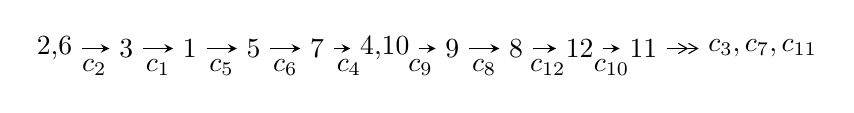
\begin{tikzpicture}[x=23pt, y=7pt]
	% node
	\node (A0) at (-1/8, 0) {2,6};
	\node (A1) at (1, 0) {3};
	\node (A2) at (2, 0) {1};
	\node (A3) at (3, 0) {5};
	\node (A4) at (4, 0) {7};
	\node (A5) at (81/16, 0) {4,10};
	\node (A6) at (49/8, 0) {9};
	\node (A7) at (57/8, 0) {8};
	\node (A8) at (65/8, 0) {12};
	\node (A9) at (73/8, 0) {11};
	\node (C1) at (1/2, -1) {$c_{2}$};
	\node (C2) at (3/2, -1) {$c_{1}$};
	\node (C3) at (5/2, -1) {$c_{5}$};
	\node (C4) at (7/2, -1) {$c_{6}$};
	\node (C5) at (9/2, -1) {$c_{4}$};
	\node (C6) at (45/8, -1) {$c_{9}$};
	\node (C7) at (53/8, -1) {$c_{8}$};
	\node (C8) at (61/8, -1) {$c_{12}$};
	\node (C9) at (69/8, -1) {$c_{10}$};
	\node (A10) at (11, 0) {$c_{3},c_{7},c_{11}$};

	% edge
	\draw[->,>=stealth]	
	(A0) edge (A1) (A1) edge (A2) (A2) edge (A3) (A3) edge (A4) (A4) edge (A5) (A5) edge (A6) (A6) edge (A7) (A7) edge (A8) (A8) edge (A9) ;
	\draw[->>,>={angle 60}]	
	(A9) edge (A10);
\end{tikzpicture} \\ 

\end{tabular} \\

\footnotetext{
The image of knot diagram is generated by the software ``\textbf{Draw programme}" developed by Andrew Bartholomew(\url{http://www.layer8.co.uk/maths/draw/index.htm\#Running-draw}), where we modified some parts for our purpose(\url{https://github.com/CATsTAILs/LinksPainter}).
}\phantom \\ \newline 
\centering \textbf{Ideals for irreducible components\footnotemark of $X_{\text{par}}$} 
 
\begin{align*}
I^u_{1}&=\langle 
- u^9+u^7- u^6-3 u^5+2 u^3+b- u,\;u^{12}- u^{10}+5 u^8-4 u^6+6 u^4-3 u^2+a- u+2,\\
\phantom{I^u_{1}}&\phantom{= \langle  }u^{13}- u^{12}- u^{11}+2 u^{10}+4 u^9-5 u^8-3 u^7+6 u^6+4 u^5-6 u^4-2 u^3+2 u^2+2 u-1\rangle \\
I^u_{2}&=\langle 
-3 u^{47}+17 u^{46}+\cdots+2 b+1,\;-11 u^{47}+29 u^{46}+\cdots+2 a+3,\;u^{48}-3 u^{47}+\cdots-2 u+1\rangle \\
I^u_{3}&=\langle 
b+u,\;a+u,\;u^3+u^2-1\rangle \\
I^u_{4}&=\langle 
b- a,\;u^2 a+a^2+u^2+2 u+1,\;u^3+u^2-1\rangle \\
\\
\end{align*}
\raggedright * 4 irreducible components of $\dim_{\mathbb{C}}=0$, with total 70 representations.\\
\footnotetext{All coefficients of polynomials are rational numbers. But the coefficients are sometimes approximated in decimal forms when there is not enough margin.}
\newpage
\renewcommand{\arraystretch}{1}
\centering \section*{I. $I^u_{1}= \langle - u^9+u^7- u^6-3 u^5+2 u^3+b- u,\;u^{12}- u^{10}+5 u^8-4 u^6+6 u^4-3 u^2+a- u+2,\;u^{13}- u^{12}+\cdots+2 u-1 \rangle$}
\flushleft \textbf{(i) Arc colorings}\\
\begin{tabular}{m{7pt} m{180pt} m{7pt} m{180pt} }
\flushright $a_{2}=$&$\begin{pmatrix}1\\0\end{pmatrix}$ \\
\flushright $a_{6}=$&$\begin{pmatrix}0\\u\end{pmatrix}$ \\
\flushright $a_{3}=$&$\begin{pmatrix}1\\u^2\end{pmatrix}$ \\
\flushright $a_{1}=$&$\begin{pmatrix}- u^2+1\\- u^4\end{pmatrix}$ \\
\flushright $a_{5}=$&$\begin{pmatrix}u\\u\end{pmatrix}$ \\
\flushright $a_{7}=$&$\begin{pmatrix}- u^3\\- u^3+u\end{pmatrix}$ \\
\flushright $a_{4}=$&$\begin{pmatrix}u^5+u\\u^5- u^3+u\end{pmatrix}$ \\
\flushright $a_{10}=$&$\begin{pmatrix}- u^{12}+u^{10}-5 u^8+4 u^6-6 u^4+3 u^2+u-2\\u^9- u^7+u^6+3 u^5-2 u^3+u\end{pmatrix}$ \\
\flushright $a_{9}=$&$\begin{pmatrix}- u^{12}+u^{10}-5 u^8+4 u^6-7 u^4+4 u^2+u-2\\u^9- u^7+3 u^5-2 u^3+u\end{pmatrix}$ \\
\flushright $a_{8}=$&$\begin{pmatrix}- u^8+u^6- u^5-3 u^4+2 u^2-1\\u^{12}-2 u^{10}+u^9+5 u^8- u^7-6 u^6+2 u^5+6 u^4- u^3-3 u^2+1\end{pmatrix}$ \\
\flushright $a_{12}=$&$\begin{pmatrix}u^{12}- u^{11}- u^{10}+u^9+4 u^8-3 u^7-4 u^6+2 u^5+5 u^4- u^3-3 u^2- u+2\\- u^{11}+u^9- u^8-3 u^7+2 u^5- u^4- u^3\end{pmatrix}$ \\
\flushright $a_{11}=$&$\begin{pmatrix}- u^{12}+u^{11}+u^{10}-2 u^9-4 u^8+4 u^7+3 u^6-5 u^5-5 u^4+3 u^3+3 u^2-2\\u^{12}- u^{10}+5 u^8-4 u^6+6 u^4-2 u^2- u+1\end{pmatrix}$\\&\end{tabular}
\flushleft \textbf{(ii) Obstruction class $= -1$}\\~\\
\flushleft \textbf{(iii) Cusp Shapes $= 4 u^{12}-2 u^{10}+18 u^8+2 u^7-6 u^6-4 u^5+20 u^4+6 u^3-2 u^2-12 u-6$}\\~\\
\newpage\renewcommand{\arraystretch}{1}
\flushleft \textbf{(iv) u-Polynomials at the component}\newline \\
\begin{tabular}{m{50pt}|m{274pt}}
Crossings & \hspace{64pt}u-Polynomials at each crossing \\
\hline $$\begin{aligned}c_{1},c_{4},c_{6}\\c_{9},c_{10},c_{12}\end{aligned}$$&$\begin{aligned}
&u^{13}+3 u^{12}+\cdots+8 u+1
\end{aligned}$\\
\hline $$\begin{aligned}c_{2},c_{5},c_{7}\\c_{11}\end{aligned}$$&$\begin{aligned}
&u^{13}+u^{12}+\cdots+2 u+1
\end{aligned}$\\
\hline $$\begin{aligned}c_{3},c_{8}\end{aligned}$$&$\begin{aligned}
&u^{13}-7 u^{12}+\cdots-24 u+8
\end{aligned}$\\
\hline
\end{tabular}\\~\\
\newpage\renewcommand{\arraystretch}{1}
\flushleft \textbf{(v) Riley Polynomials at the component}\newline \\
\begin{tabular}{m{50pt}|m{274pt}}
Crossings & \hspace{64pt}Riley Polynomials at each crossing \\
\hline $$\begin{aligned}c_{1},c_{4},c_{6}\\c_{9},c_{10},c_{12}\end{aligned}$$&$\begin{aligned}
&y^{13}+17 y^{12}+\cdots+16 y-1
\end{aligned}$\\
\hline $$\begin{aligned}c_{2},c_{5},c_{7}\\c_{11}\end{aligned}$$&$\begin{aligned}
&y^{13}-3 y^{12}+\cdots+8 y-1
\end{aligned}$\\
\hline $$\begin{aligned}c_{3},c_{8}\end{aligned}$$&$\begin{aligned}
&y^{13}+7 y^{12}+\cdots+128 y-64
\end{aligned}$\\
\hline
\end{tabular}\\~\\
\newpage\flushleft \textbf{(vi) Complex Volumes and Cusp Shapes}
$$\begin{array}{c|c|c}  
\text{Solutions to }I^u_{1}& \I (\text{vol} + \sqrt{-1}CS) & \text{Cusp shape}\\
 \hline 
\begin{aligned}
u &= -0.923828 + 0.421970 I \\
a &= \phantom{-}0.763252 + 0.399422 I \\
b &= \phantom{-}0.261288 - 0.366463 I\end{aligned}
 & -0.05055 + 6.40816 I & -12.2349 - 10.2893 I \\ \hline\begin{aligned}
u &= -0.923828 - 0.421970 I \\
a &= \phantom{-}0.763252 - 0.399422 I \\
b &= \phantom{-}0.261288 + 0.366463 I\end{aligned}
 & -0.05055 - 6.40816 I & -12.2349 + 10.2893 I \\ \hline\begin{aligned}
u &= \phantom{-}0.801388 + 0.281223 I \\
a &= \phantom{-}0.268761 - 0.576127 I \\
b &= -0.168515 + 0.695868 I\end{aligned}
 & -2.04094 - 2.18131 I & -16.1482 + 7.3921 I \\ \hline\begin{aligned}
u &= \phantom{-}0.801388 - 0.281223 I \\
a &= \phantom{-}0.268761 + 0.576127 I \\
b &= -0.168515 - 0.695868 I\end{aligned}
 & -2.04094 + 2.18131 I & -16.1482 - 7.3921 I \\ \hline\begin{aligned}
u &= -0.537404 + 0.591513 I \\
a &= -0.786204 - 0.602557 I \\
b &= -0.632206 - 0.390230 I\end{aligned}
 & \phantom{-}2.68260 + 1.42666 I & -3.83184 - 3.78939 I \\ \hline\begin{aligned}
u &= -0.537404 - 0.591513 I \\
a &= -0.786204 + 0.602557 I \\
b &= -0.632206 + 0.390230 I\end{aligned}
 & \phantom{-}2.68260 - 1.42666 I & -3.83184 + 3.78939 I \\ \hline\begin{aligned}
u &= \phantom{-}0.855993 + 0.936945 I \\
a &= -3.04281 - 0.69376 I \\
b &= -1.58297 - 3.59981 I\end{aligned}
 & \phantom{-}18.0409 + 0.9847 I & -4.10351 + 1.46024 I \\ \hline\begin{aligned}
u &= \phantom{-}0.855993 - 0.936945 I \\
a &= -3.04281 + 0.69376 I \\
b &= -1.58297 + 3.59981 I\end{aligned}
 & \phantom{-}18.0409 - 0.9847 I & -4.10351 - 1.46024 I \\ \hline\begin{aligned}
u &= -0.928636 + 0.877531 I \\
a &= -3.22583 + 2.14654 I \\
b &= -0.92820 + 5.06333 I\end{aligned}
 & \phantom{-}12.42090 + 6.50749 I & -5.85522 - 4.78409 I \\ \hline\begin{aligned}
u &= -0.928636 - 0.877531 I \\
a &= -3.22583 - 2.14654 I \\
b &= -0.92820 - 5.06333 I\end{aligned}
 & \phantom{-}12.42090 - 6.50749 I & -5.85522 + 4.78409 I\\
 \hline 
 \end{array}$$\newpage$$\begin{array}{c|c|c}  
\text{Solutions to }I^u_{1}& \I (\text{vol} + \sqrt{-1}CS) & \text{Cusp shape}\\
 \hline 
\begin{aligned}
u &= \phantom{-}1.002580 + 0.857613 I \\
a &= -1.90418 - 2.60319 I \\
b &= \phantom{-}0.38407 - 4.60433 I\end{aligned}
 & \phantom{-}17.0728 - 14.2174 I & -5.54739 + 7.80237 I \\ \hline\begin{aligned}
u &= \phantom{-}1.002580 - 0.857613 I \\
a &= -1.90418 + 2.60319 I \\
b &= \phantom{-}0.38407 + 4.60433 I\end{aligned}
 & \phantom{-}17.0728 + 14.2174 I & -5.54739 - 7.80237 I \\ \hline\begin{aligned}
u &= \phantom{-}0.459806\phantom{ +0.000000I} \\
a &= -1.14598\phantom{ +0.000000I} \\
b &= \phantom{-}0.333063\phantom{ +0.000000I}\end{aligned}
 & -0.845259\phantom{ +0.000000I} & -10.5580\phantom{ +0.000000I}\\
 \hline 
 \end{array}$$\newpage\newpage\renewcommand{\arraystretch}{1}
\centering \section*{II. $I^u_{2}= \langle -3 u^{47}+17 u^{46}+\cdots+2 b+1,\;-11 u^{47}+29 u^{46}+\cdots+2 a+3,\;u^{48}-3 u^{47}+\cdots-2 u+1 \rangle$}
\flushleft \textbf{(i) Arc colorings}\\
\begin{tabular}{m{7pt} m{180pt} m{7pt} m{180pt} }
\flushright $a_{2}=$&$\begin{pmatrix}1\\0\end{pmatrix}$ \\
\flushright $a_{6}=$&$\begin{pmatrix}0\\u\end{pmatrix}$ \\
\flushright $a_{3}=$&$\begin{pmatrix}1\\u^2\end{pmatrix}$ \\
\flushright $a_{1}=$&$\begin{pmatrix}- u^2+1\\- u^4\end{pmatrix}$ \\
\flushright $a_{5}=$&$\begin{pmatrix}u\\u\end{pmatrix}$ \\
\flushright $a_{7}=$&$\begin{pmatrix}- u^3\\- u^3+u\end{pmatrix}$ \\
\flushright $a_{4}=$&$\begin{pmatrix}u^5+u\\u^5- u^3+u\end{pmatrix}$ \\
\flushright $a_{10}=$&$\begin{pmatrix}\frac{11}{2} u^{47}-\frac{29}{2} u^{46}+\cdots-\frac{17}{2} u-\frac{3}{2}\\\frac{3}{2} u^{47}-\frac{17}{2} u^{46}+\cdots-\frac{7}{2} u-\frac{1}{2}\end{pmatrix}$ \\
\flushright $a_{9}=$&$\begin{pmatrix}\frac{17}{2} u^{47}-23 u^{46}+\cdots-9 u-\frac{5}{2}\\2 u^{47}-\frac{27}{2} u^{46}+\cdots-\frac{1}{2} u-\frac{7}{2}\end{pmatrix}$ \\
\flushright $a_{8}=$&$\begin{pmatrix}-\frac{1}{2} u^{47}+9 u^{45}+\cdots-19 u+\frac{9}{2}\\-2 u^{47}+\frac{13}{2} u^{46}+\cdots-\frac{19}{2} u+\frac{11}{2}\end{pmatrix}$ \\
\flushright $a_{12}=$&$\begin{pmatrix}-\frac{1}{2} u^{45}+u^{44}+\cdots+\frac{7}{2} u^2+\frac{3}{2}\\-\frac{1}{2} u^{45}+u^{44}+\cdots+\frac{15}{2} u^2-\frac{1}{2}\end{pmatrix}$ \\
\flushright $a_{11}=$&$\begin{pmatrix}-\frac{1}{2} u^{47}+3 u^{46}+\cdots+7 u-5\\-\frac{1}{2} u^{46}- u^{45}+\cdots+\frac{13}{2} u-2\end{pmatrix}$\\&\end{tabular}
\flushleft \textbf{(ii) Obstruction class $= -1$}\\~\\
\flushleft \textbf{(iii) Cusp Shapes $= - u^{47}+\frac{23}{2} u^{46}+\cdots-\frac{77}{2} u+\frac{11}{2}$}\\~\\
\newpage\renewcommand{\arraystretch}{1}
\flushleft \textbf{(iv) u-Polynomials at the component}\newline \\
\begin{tabular}{m{50pt}|m{274pt}}
Crossings & \hspace{64pt}u-Polynomials at each crossing \\
\hline $$\begin{aligned}c_{1},c_{4},c_{6}\\c_{9},c_{10},c_{12}\end{aligned}$$&$\begin{aligned}
&u^{48}+11 u^{47}+\cdots+28 u+1
\end{aligned}$\\
\hline $$\begin{aligned}c_{2},c_{5},c_{7}\\c_{11}\end{aligned}$$&$\begin{aligned}
&u^{48}+3 u^{47}+\cdots+2 u+1
\end{aligned}$\\
\hline $$\begin{aligned}c_{3},c_{8}\end{aligned}$$&$\begin{aligned}
&(u^{24}+3 u^{23}+\cdots+20 u+8)^{2}
\end{aligned}$\\
\hline
\end{tabular}\\~\\
\newpage\renewcommand{\arraystretch}{1}
\flushleft \textbf{(v) Riley Polynomials at the component}\newline \\
\begin{tabular}{m{50pt}|m{274pt}}
Crossings & \hspace{64pt}Riley Polynomials at each crossing \\
\hline $$\begin{aligned}c_{1},c_{4},c_{6}\\c_{9},c_{10},c_{12}\end{aligned}$$&$\begin{aligned}
&y^{48}+53 y^{47}+\cdots-188 y+1
\end{aligned}$\\
\hline $$\begin{aligned}c_{2},c_{5},c_{7}\\c_{11}\end{aligned}$$&$\begin{aligned}
&y^{48}-11 y^{47}+\cdots-28 y+1
\end{aligned}$\\
\hline $$\begin{aligned}c_{3},c_{8}\end{aligned}$$&$\begin{aligned}
&(y^{24}+21 y^{23}+\cdots+496 y+64)^{2}
\end{aligned}$\\
\hline
\end{tabular}\\~\\
\newpage\flushleft \textbf{(vi) Complex Volumes and Cusp Shapes}
$$\begin{array}{c|c|c}  
\text{Solutions to }I^u_{2}& \I (\text{vol} + \sqrt{-1}CS) & \text{Cusp shape}\\
 \hline 
\begin{aligned}
u &= -0.841794 + 0.516230 I \\
a &= -0.724878 - 0.760407 I \\
b &= -0.543660 - 0.322602 I\end{aligned}
 & \phantom{-}1.74731 + 2.75249 I & -5.85663 - 4.25990 I \\ \hline\begin{aligned}
u &= -0.841794 - 0.516230 I \\
a &= -0.724878 + 0.760407 I \\
b &= -0.543660 + 0.322602 I\end{aligned}
 & \phantom{-}1.74731 - 2.75249 I & -5.85663 + 4.25990 I \\ \hline\begin{aligned}
u &= \phantom{-}0.930322 + 0.093737 I \\
a &= \phantom{-}0.274062 - 0.684145 I \\
b &= \phantom{-}0.528392 - 0.143631 I\end{aligned}
 & -1.87399 + 1.33150 I & -14.6087 - 4.8388 I \\ \hline\begin{aligned}
u &= \phantom{-}0.930322 - 0.093737 I \\
a &= \phantom{-}0.274062 + 0.684145 I \\
b &= \phantom{-}0.528392 + 0.143631 I\end{aligned}
 & -1.87399 - 1.33150 I & -14.6087 + 4.8388 I \\ \hline\begin{aligned}
u &= \phantom{-}1.074940 + 0.011887 I \\
a &= \phantom{-}0.08400 - 1.42217 I \\
b &= \phantom{-}0.24511 - 2.16612 I\end{aligned}
 & \phantom{-}5.18079 + 3.17559 I & -10.00740 - 2.50769 I \\ \hline\begin{aligned}
u &= \phantom{-}1.074940 - 0.011887 I \\
a &= \phantom{-}0.08400 + 1.42217 I \\
b &= \phantom{-}0.24511 + 2.16612 I\end{aligned}
 & \phantom{-}5.18079 - 3.17559 I & -10.00740 + 2.50769 I \\ \hline\begin{aligned}
u &= \phantom{-}0.746614 + 0.498009 I \\
a &= -0.183156 - 1.279540 I \\
b &= -1.014170 + 0.309519 I\end{aligned}
 & \phantom{-}4.20175 - 4.96532 I & -9.50591 + 5.64619 I \\ \hline\begin{aligned}
u &= \phantom{-}0.746614 - 0.498009 I \\
a &= -0.183156 + 1.279540 I \\
b &= -1.014170 - 0.309519 I\end{aligned}
 & \phantom{-}4.20175 + 4.96532 I & -9.50591 - 5.64619 I \\ \hline\begin{aligned}
u &= -0.366415 + 0.805565 I \\
a &= -1.17167 + 1.18416 I \\
b &= \phantom{-}0.184920 - 0.596372 I\end{aligned}
 & \phantom{-}10.50330 + 1.42992 I & -3.65523 - 2.00550 I \\ \hline\begin{aligned}
u &= -0.366415 - 0.805565 I \\
a &= -1.17167 - 1.18416 I \\
b &= \phantom{-}0.184920 + 0.596372 I\end{aligned}
 & \phantom{-}10.50330 - 1.42992 I & -3.65523 + 2.00550 I\\
 \hline 
 \end{array}$$\newpage$$\begin{array}{c|c|c}  
\text{Solutions to }I^u_{2}& \I (\text{vol} + \sqrt{-1}CS) & \text{Cusp shape}\\
 \hline 
\begin{aligned}
u &= -0.336222 + 0.803215 I \\
a &= \phantom{-}0.87556 - 1.36537 I \\
b &= -0.137852 + 0.789514 I\end{aligned}
 & \phantom{-}10.34730 - 5.08751 I & -3.92984 + 2.90656 I \\ \hline\begin{aligned}
u &= -0.336222 - 0.803215 I \\
a &= \phantom{-}0.87556 + 1.36537 I \\
b &= -0.137852 - 0.789514 I\end{aligned}
 & \phantom{-}10.34730 + 5.08751 I & -3.92984 - 2.90656 I \\ \hline\begin{aligned}
u &= -0.880758 + 0.714367 I \\
a &= -0.556508 - 0.593812 I \\
b &= -0.762556 - 0.329885 I\end{aligned}
 & \phantom{-}2.31973 + 2.73395 I & \phantom{-0.000000 }      -6
0. 10   - 0.676902 I \\ \hline\begin{aligned}
u &= -0.880758 - 0.714367 I \\
a &= -0.556508 + 0.593812 I \\
b &= -0.762556 + 0.329885 I\end{aligned}
 & \phantom{-}2.31973 - 2.73395 I & \phantom{-0.000000 -}     -6
0. 10   + 0.676902 I \\ \hline\begin{aligned}
u &= \phantom{-}0.696228 + 0.511765 I \\
a &= -0.02775 + 1.48585 I \\
b &= \phantom{-}0.840769 - 0.158612 I\end{aligned}
 & \phantom{-}4.36673 + 1.08082 I & -8.65197 + 0.09587 I \\ \hline\begin{aligned}
u &= \phantom{-}0.696228 - 0.511765 I \\
a &= -0.02775 - 1.48585 I \\
b &= \phantom{-}0.840769 + 0.158612 I\end{aligned}
 & \phantom{-}4.36673 - 1.08082 I & -8.65197 - 0.09587 I \\ \hline\begin{aligned}
u &= -1.040760 + 0.477829 I \\
a &= -0.022096 + 0.260934 I \\
b &= -1.60902 + 0.01527 I\end{aligned}
 & \phantom{-}8.01455 + 9.71739 I & -7.98988 - 8.06760 I \\ \hline\begin{aligned}
u &= -1.040760 - 0.477829 I \\
a &= -0.022096 - 0.260934 I \\
b &= -1.60902 - 0.01527 I\end{aligned}
 & \phantom{-}8.01455 - 9.71739 I & -7.98988 + 8.06760 I \\ \hline\begin{aligned}
u &= -1.035350 + 0.498737 I \\
a &= \phantom{-}0.036384 - 0.448348 I \\
b &= \phantom{-}1.46608 - 0.47696 I\end{aligned}
 & \phantom{-}8.29415 + 3.29720 I & -7.24610 - 3.17160 I \\ \hline\begin{aligned}
u &= -1.035350 - 0.498737 I \\
a &= \phantom{-}0.036384 + 0.448348 I \\
b &= \phantom{-}1.46608 + 0.47696 I\end{aligned}
 & \phantom{-}8.29415 - 3.29720 I & -7.24610 + 3.17160 I\\
 \hline 
 \end{array}$$\newpage$$\begin{array}{c|c|c}  
\text{Solutions to }I^u_{2}& \I (\text{vol} + \sqrt{-1}CS) & \text{Cusp shape}\\
 \hline 
\begin{aligned}
u &= -0.751107 + 0.340936 I \\
a &= \phantom{-}1.07827 + 0.93654 I \\
b &= \phantom{-}1.136920 + 0.261943 I\end{aligned}
 & -1.87399 + 1.33150 I & -14.6087 - 4.8388 I \\ \hline\begin{aligned}
u &= -0.751107 - 0.340936 I \\
a &= \phantom{-}1.07827 - 0.93654 I \\
b &= \phantom{-}1.136920 - 0.261943 I\end{aligned}
 & -1.87399 - 1.33150 I & -14.6087 + 4.8388 I \\ \hline\begin{aligned}
u &= -0.864737 + 0.816422 I \\
a &= \phantom{-}1.00270 - 1.60989 I \\
b &= -0.28591 - 2.01649 I\end{aligned}
 & \phantom{-}4.36673 + 1.08082 I & -8.65197 + 0. I\phantom{ +0.000000I} \\ \hline\begin{aligned}
u &= -0.864737 - 0.816422 I \\
a &= \phantom{-}1.00270 + 1.60989 I \\
b &= -0.28591 + 2.01649 I\end{aligned}
 & \phantom{-}4.36673 - 1.08082 I & -8.65197 + 0. I\phantom{ +0.000000I} \\ \hline\begin{aligned}
u &= -0.917877 + 0.800067 I \\
a &= -1.77023 + 0.64969 I \\
b &= -1.31308 + 1.88984 I\end{aligned}
 & \phantom{-}4.20175 + 4.96532 I & -12.00000 - 5.64619 I \\ \hline\begin{aligned}
u &= -0.917877 - 0.800067 I \\
a &= -1.77023 - 0.64969 I \\
b &= -1.31308 - 1.88984 I\end{aligned}
 & \phantom{-}4.20175 - 4.96532 I & -12.00000 + 5.64619 I \\ \hline\begin{aligned}
u &= \phantom{-}0.871124 + 0.885192 I \\
a &= \phantom{-}1.28643 + 0.63717 I \\
b &= \phantom{-}0.88470 + 1.89792 I\end{aligned}
 & \phantom{-}8.29415 + 3.29720 I & -12.00000 + 0. I\phantom{ +0.000000I} \\ \hline\begin{aligned}
u &= \phantom{-}0.871124 - 0.885192 I \\
a &= \phantom{-}1.28643 - 0.63717 I \\
b &= \phantom{-}0.88470 - 1.89792 I\end{aligned}
 & \phantom{-}8.29415 - 3.29720 I & -12.00000 + 0. I\phantom{ +0.000000I} \\ \hline\begin{aligned}
u &= \phantom{-}0.913300 + 0.855274 I \\
a &= -0.195582 - 0.163086 I \\
b &= \phantom{-}0.346423 + 0.202860 I\end{aligned}
 & \phantom{-}5.18079 - 3.17559 I & -12.00000 + 0. I\phantom{ +0.000000I} \\ \hline\begin{aligned}
u &= \phantom{-}0.913300 - 0.855274 I \\
a &= -0.195582 + 0.163086 I \\
b &= \phantom{-}0.346423 - 0.202860 I\end{aligned}
 & \phantom{-}5.18079 + 3.17559 I & -12.00000 + 0. I\phantom{ +0.000000I}\\
 \hline 
 \end{array}$$\newpage$$\begin{array}{c|c|c}  
\text{Solutions to }I^u_{2}& \I (\text{vol} + \sqrt{-1}CS) & \text{Cusp shape}\\
 \hline 
\begin{aligned}
u &= \phantom{-}0.845587 + 0.935523 I \\
a &= \phantom{-}3.03496 + 1.05311 I \\
b &= \phantom{-}1.18613 + 3.70268 I\end{aligned}
 & \phantom{-}17.5794 + 7.6165 I & -12.00000 + 0. I\phantom{ +0.000000I} \\ \hline\begin{aligned}
u &= \phantom{-}0.845587 - 0.935523 I \\
a &= \phantom{-}3.03496 - 1.05311 I \\
b &= \phantom{-}1.18613 - 3.70268 I\end{aligned}
 & \phantom{-}17.5794 - 7.6165 I & -12.00000 + 0. I\phantom{ +0.000000I} \\ \hline\begin{aligned}
u &= \phantom{-}0.898811 + 0.892925 I \\
a &= -1.169680 + 0.302901 I \\
b &= -1.61570 - 1.19571 I\end{aligned}
 & \phantom{-}10.50330 - 1.42992 I & -12.00000 + 0. I\phantom{ +0.000000I} \\ \hline\begin{aligned}
u &= \phantom{-}0.898811 - 0.892925 I \\
a &= -1.169680 - 0.302901 I \\
b &= -1.61570 + 1.19571 I\end{aligned}
 & \phantom{-}10.50330 + 1.42992 I & -12.00000 + 0. I\phantom{ +0.000000I} \\ \hline\begin{aligned}
u &= -0.917895 + 0.882530 I \\
a &= \phantom{-}3.01654 - 2.45632 I \\
b &= \phantom{-}0.32556 - 5.04361 I\end{aligned}
 & \phantom{-}12.4555\phantom{ +0.000000I} & \phantom{-0.000000 } 0 \\ \hline\begin{aligned}
u &= -0.917895 - 0.882530 I \\
a &= \phantom{-}3.01654 + 2.45632 I \\
b &= \phantom{-}0.32556 + 5.04361 I\end{aligned}
 & \phantom{-}12.4555\phantom{ +0.000000I} & \phantom{-0.000000 } 0 \\ \hline\begin{aligned}
u &= \phantom{-}0.959444 + 0.848413 I \\
a &= -1.18514 - 1.34955 I \\
b &= \phantom{-}0.10952 - 1.97053 I\end{aligned}
 & \phantom{-}8.01455 - 9.71739 I & \phantom{-0.000000 } 0 \\ \hline\begin{aligned}
u &= \phantom{-}0.959444 - 0.848413 I \\
a &= -1.18514 + 1.34955 I \\
b &= \phantom{-}0.10952 + 1.97053 I\end{aligned}
 & \phantom{-}8.01455 + 9.71739 I & \phantom{-0.000000 } 0 \\ \hline\begin{aligned}
u &= \phantom{-}0.947556 + 0.870745 I \\
a &= \phantom{-}0.33672 + 1.44236 I \\
b &= -1.26760 + 1.29298 I\end{aligned}
 & \phantom{-}10.34730 - 5.08751 I & \phantom{-0.000000 } 0 \\ \hline\begin{aligned}
u &= \phantom{-}0.947556 - 0.870745 I \\
a &= \phantom{-}0.33672 - 1.44236 I \\
b &= -1.26760 - 1.29298 I\end{aligned}
 & \phantom{-}10.34730 + 5.08751 I & \phantom{-0.000000 } 0\\
 \hline 
 \end{array}$$\newpage$$\begin{array}{c|c|c}  
\text{Solutions to }I^u_{2}& \I (\text{vol} + \sqrt{-1}CS) & \text{Cusp shape}\\
 \hline 
\begin{aligned}
u &= \phantom{-}0.998762 + 0.865177 I \\
a &= \phantom{-}1.62848 + 2.70839 I \\
b &= -0.93674 + 4.41906 I\end{aligned}
 & \phantom{-}17.5794 - 7.6165 I & \phantom{-0.000000 } 0 \\ \hline\begin{aligned}
u &= \phantom{-}0.998762 - 0.865177 I \\
a &= \phantom{-}1.62848 - 2.70839 I \\
b &= -0.93674 - 4.41906 I\end{aligned}
 & \phantom{-}17.5794 + 7.6165 I & \phantom{-0.000000 } 0 \\ \hline\begin{aligned}
u &= -0.304534 + 0.542389 I \\
a &= -0.125842 + 0.286126 I \\
b &= \phantom{-}0.557583 + 0.600347 I\end{aligned}
 & \phantom{-}1.74731 - 2.75249 I & -5.85663 + 4.25990 I \\ \hline\begin{aligned}
u &= -0.304534 - 0.542389 I \\
a &= -0.125842 - 0.286126 I \\
b &= \phantom{-}0.557583 - 0.600347 I\end{aligned}
 & \phantom{-}1.74731 + 2.75249 I & -5.85663 - 4.25990 I \\ \hline\begin{aligned}
u &= \phantom{-}0.579212\phantom{ +0.000000I} \\
a &= -0.784912\phantom{ +0.000000I} \\
b &= \phantom{-}0.245364\phantom{ +0.000000I}\end{aligned}
 & -0.838576\phantom{ +0.000000I} & -11.3810\phantom{ +0.000000I} \\ \hline\begin{aligned}
u &= -0.551506 + 0.061917 I \\
a &= \phantom{-}0.27580 + 2.18978 I \\
b &= \phantom{-}0.36476 + 1.51138 I\end{aligned}
 & \phantom{-}2.31973 - 2.73395 I & \phantom{-}0.279102 + 0.676902 I \\ \hline\begin{aligned}
u &= -0.551506 - 0.061917 I \\
a &= \phantom{-}0.27580 - 2.18978 I \\
b &= \phantom{-}0.36476 - 1.51138 I\end{aligned}
 & \phantom{-}2.31973 + 2.73395 I & \phantom{-}0.279102 - 0.676902 I \\ \hline\begin{aligned}
u &= \phantom{-}0.273323\phantom{ +0.000000I} \\
a &= -1.80982\phantom{ +0.000000I} \\
b &= \phantom{-}0.373488\phantom{ +0.000000I}\end{aligned}
 & -0.838576\phantom{ +0.000000I} & -11.3810\phantom{ +0.000000I}\\
 \hline 
 \end{array}$$\newpage\newpage\renewcommand{\arraystretch}{1}
\centering \section*{III. $I^u_{3}= \langle b+u,\;a+u,\;u^3+u^2-1 \rangle$}
\flushleft \textbf{(i) Arc colorings}\\
\begin{tabular}{m{7pt} m{180pt} m{7pt} m{180pt} }
\flushright $a_{2}=$&$\begin{pmatrix}1\\0\end{pmatrix}$ \\
\flushright $a_{6}=$&$\begin{pmatrix}0\\u\end{pmatrix}$ \\
\flushright $a_{3}=$&$\begin{pmatrix}1\\u^2\end{pmatrix}$ \\
\flushright $a_{1}=$&$\begin{pmatrix}- u^2+1\\- u^2- u+1\end{pmatrix}$ \\
\flushright $a_{5}=$&$\begin{pmatrix}u\\u\end{pmatrix}$ \\
\flushright $a_{7}=$&$\begin{pmatrix}u^2-1\\u^2+u-1\end{pmatrix}$ \\
\flushright $a_{4}=$&$\begin{pmatrix}1\\u^2\end{pmatrix}$ \\
\flushright $a_{10}=$&$\begin{pmatrix}- u\\- u\end{pmatrix}$ \\
\flushright $a_{9}=$&$\begin{pmatrix}-1\\- u^2\end{pmatrix}$ \\
\flushright $a_{8}=$&$\begin{pmatrix}-1\\- u^2\end{pmatrix}$ \\
\flushright $a_{12}=$&$\begin{pmatrix}0\\- u\end{pmatrix}$ \\
\flushright $a_{11}=$&$\begin{pmatrix}- u\\u^2- u-1\end{pmatrix}$\\&\end{tabular}
\flushleft \textbf{(ii) Obstruction class $= 1$}\\~\\
\flushleft \textbf{(iii) Cusp Shapes $= -8 u-12$}\\~\\
\newpage\renewcommand{\arraystretch}{1}
\flushleft \textbf{(iv) u-Polynomials at the component}\newline \\
\begin{tabular}{m{50pt}|m{274pt}}
Crossings & \hspace{64pt}u-Polynomials at each crossing \\
\hline $$\begin{aligned}c_{1},c_{4},c_{9}\\c_{10}\end{aligned}$$&$\begin{aligned}
&u^3- u^2+2 u-1
\end{aligned}$\\
\hline $$\begin{aligned}c_{2},c_{7}\end{aligned}$$&$\begin{aligned}
&u^3+u^2-1
\end{aligned}$\\
\hline $$\begin{aligned}c_{3},c_{8}\end{aligned}$$&$\begin{aligned}
&u^3
\end{aligned}$\\
\hline $$\begin{aligned}c_{5},c_{11}\end{aligned}$$&$\begin{aligned}
&u^3- u^2+1
\end{aligned}$\\
\hline $$\begin{aligned}c_{6},c_{12}\end{aligned}$$&$\begin{aligned}
&u^3+u^2+2 u+1
\end{aligned}$\\
\hline
\end{tabular}\\~\\
\newpage\renewcommand{\arraystretch}{1}
\flushleft \textbf{(v) Riley Polynomials at the component}\newline \\
\begin{tabular}{m{50pt}|m{274pt}}
Crossings & \hspace{64pt}Riley Polynomials at each crossing \\
\hline $$\begin{aligned}c_{1},c_{4},c_{6}\\c_{9},c_{10},c_{12}\end{aligned}$$&$\begin{aligned}
&y^3+3 y^2+2 y-1
\end{aligned}$\\
\hline $$\begin{aligned}c_{2},c_{5},c_{7}\\c_{11}\end{aligned}$$&$\begin{aligned}
&y^3- y^2+2 y-1
\end{aligned}$\\
\hline $$\begin{aligned}c_{3},c_{8}\end{aligned}$$&$\begin{aligned}
&y^3
\end{aligned}$\\
\hline
\end{tabular}\\~\\
\newpage\flushleft \textbf{(vi) Complex Volumes and Cusp Shapes}
$$\begin{array}{c|c|c}  
\text{Solutions to }I^u_{3}& \I (\text{vol} + \sqrt{-1}CS) & \text{Cusp shape}\\
 \hline 
\begin{aligned}
u &= -0.877439 + 0.744862 I \\
a &= \phantom{-}0.877439 - 0.744862 I \\
b &= \phantom{-}0.877439 - 0.744862 I\end{aligned}
 & \phantom{-}6.04826 + 5.65624 I & -4.98049 - 5.95889 I \\ \hline\begin{aligned}
u &= -0.877439 - 0.744862 I \\
a &= \phantom{-}0.877439 + 0.744862 I \\
b &= \phantom{-}0.877439 + 0.744862 I\end{aligned}
 & \phantom{-}6.04826 - 5.65624 I & -4.98049 + 5.95889 I \\ \hline\begin{aligned}
u &= \phantom{-}0.754878\phantom{ +0.000000I} \\
a &= -0.754878\phantom{ +0.000000I} \\
b &= -0.754878\phantom{ +0.000000I}\end{aligned}
 & -2.22691\phantom{ +0.000000I} & -18.0390\phantom{ +0.000000I}\\
 \hline 
 \end{array}$$\newpage\newpage\renewcommand{\arraystretch}{1}
\centering \section*{IV. $I^u_{4}= \langle b- a,\;u^2 a+a^2+u^2+2 u+1,\;u^3+u^2-1 \rangle$}
\flushleft \textbf{(i) Arc colorings}\\
\begin{tabular}{m{7pt} m{180pt} m{7pt} m{180pt} }
\flushright $a_{2}=$&$\begin{pmatrix}1\\0\end{pmatrix}$ \\
\flushright $a_{6}=$&$\begin{pmatrix}0\\u\end{pmatrix}$ \\
\flushright $a_{3}=$&$\begin{pmatrix}1\\u^2\end{pmatrix}$ \\
\flushright $a_{1}=$&$\begin{pmatrix}- u^2+1\\- u^2- u+1\end{pmatrix}$ \\
\flushright $a_{5}=$&$\begin{pmatrix}u\\u\end{pmatrix}$ \\
\flushright $a_{7}=$&$\begin{pmatrix}u^2-1\\u^2+u-1\end{pmatrix}$ \\
\flushright $a_{4}=$&$\begin{pmatrix}1\\u^2\end{pmatrix}$ \\
\flushright $a_{10}=$&$\begin{pmatrix}a\\a\end{pmatrix}$ \\
\flushright $a_{9}=$&$\begin{pmatrix}u^2 a+a u\\a u\end{pmatrix}$ \\
\flushright $a_{8}=$&$\begin{pmatrix}u^2 a+a u\\a u\end{pmatrix}$ \\
\flushright $a_{12}=$&$\begin{pmatrix}- u^2 a+a+u+2\\- u^2 a+a+2\end{pmatrix}$ \\
\flushright $a_{11}=$&$\begin{pmatrix}-2 u^2 a- a u+a+1\\- u^2 a- a u+a+1\end{pmatrix}$\\&\end{tabular}
\flushleft \textbf{(ii) Obstruction class $= 1$}\\~\\
\flushleft \textbf{(iii) Cusp Shapes $= 8 u^2 a+a u- u^2-8 a-19$}\\~\\
\newpage\renewcommand{\arraystretch}{1}
\flushleft \textbf{(iv) u-Polynomials at the component}\newline \\
\begin{tabular}{m{50pt}|m{274pt}}
Crossings & \hspace{64pt}u-Polynomials at each crossing \\
\hline $$\begin{aligned}c_{1},c_{4},c_{9}\\c_{10}\end{aligned}$$&$\begin{aligned}
&(u^3- u^2+2 u-1)^2
\end{aligned}$\\
\hline $$\begin{aligned}c_{2},c_{7}\end{aligned}$$&$\begin{aligned}
&(u^3+u^2-1)^2
\end{aligned}$\\
\hline $$\begin{aligned}c_{3},c_{8}\end{aligned}$$&$\begin{aligned}
&u^6
\end{aligned}$\\
\hline $$\begin{aligned}c_{5},c_{11}\end{aligned}$$&$\begin{aligned}
&(u^3- u^2+1)^2
\end{aligned}$\\
\hline $$\begin{aligned}c_{6},c_{12}\end{aligned}$$&$\begin{aligned}
&(u^3+u^2+2 u+1)^2
\end{aligned}$\\
\hline
\end{tabular}\\~\\
\newpage\renewcommand{\arraystretch}{1}
\flushleft \textbf{(v) Riley Polynomials at the component}\newline \\
\begin{tabular}{m{50pt}|m{274pt}}
Crossings & \hspace{64pt}Riley Polynomials at each crossing \\
\hline $$\begin{aligned}c_{1},c_{4},c_{6}\\c_{9},c_{10},c_{12}\end{aligned}$$&$\begin{aligned}
&(y^3+3 y^2+2 y-1)^2
\end{aligned}$\\
\hline $$\begin{aligned}c_{2},c_{5},c_{7}\\c_{11}\end{aligned}$$&$\begin{aligned}
&(y^3- y^2+2 y-1)^2
\end{aligned}$\\
\hline $$\begin{aligned}c_{3},c_{8}\end{aligned}$$&$\begin{aligned}
&y^6
\end{aligned}$\\
\hline
\end{tabular}\\~\\
\newpage\flushleft \textbf{(vi) Complex Volumes and Cusp Shapes}
$$\begin{array}{c|c|c}  
\text{Solutions to }I^u_{4}& \I (\text{vol} + \sqrt{-1}CS) & \text{Cusp shape}\\
 \hline 
\begin{aligned}
u &= -0.877439 + 0.744862 I \\
a &= -0.592519 + 0.986732 I \\
b &= -0.592519 + 0.986732 I\end{aligned}
 & \phantom{-}6.04826\phantom{ +0.000000I} & -5.39114 + 0. I\phantom{ +0.000000I} \\ \hline\begin{aligned}
u &= -0.877439 + 0.744862 I \\
a &= \phantom{-}0.377439 + 0.320410 I \\
b &= \phantom{-}0.377439 + 0.320410 I\end{aligned}
 & \phantom{-}1.91067 + 2.82812 I & -18.8044 - 4.6518 I \\ \hline\begin{aligned}
u &= -0.877439 - 0.744862 I \\
a &= -0.592519 - 0.986732 I \\
b &= -0.592519 - 0.986732 I\end{aligned}
 & \phantom{-}6.04826\phantom{ +0.000000I} & -5.39114 + 0. I\phantom{ +0.000000I} \\ \hline\begin{aligned}
u &= -0.877439 - 0.744862 I \\
a &= \phantom{-}0.377439 - 0.320410 I \\
b &= \phantom{-}0.377439 - 0.320410 I\end{aligned}
 & \phantom{-}1.91067 - 2.82812 I & -18.8044 + 4.6518 I \\ \hline\begin{aligned}
u &= \phantom{-}0.754878\phantom{ +0.000000I} \\
a &= -0.28492 + 1.73159 I \\
b &= -0.28492 + 1.73159 I\end{aligned}
 & \phantom{-}1.91067 + 2.82812 I & -18.8044 - 4.6518 I \\ \hline\begin{aligned}
u &= \phantom{-}0.754878\phantom{ +0.000000I} \\
a &= -0.28492 - 1.73159 I \\
b &= -0.28492 - 1.73159 I\end{aligned}
 & \phantom{-}1.91067 - 2.82812 I & -18.8044 + 4.6518 I\\
 \hline 
 \end{array}$$\newpage
\newpage\renewcommand{\arraystretch}{1}
\centering \section*{ V. u-Polynomials}
\begin{tabular}{m{50pt}|m{274pt}}
Crossings & \hspace{64pt}u-Polynomials at each crossing \\
\hline $$\begin{aligned}c_{1},c_{4},c_{9}\\c_{10}\end{aligned}$$&$\begin{aligned}
&((u^3- u^2+2 u-1)^3)(u^{13}+3 u^{12}+\cdots+8 u+1)\\
&\cdot(u^{48}+11 u^{47}+\cdots+28 u+1)
\end{aligned}$\\
\hline $$\begin{aligned}c_{2},c_{7}\end{aligned}$$&$\begin{aligned}
&((u^3+u^2-1)^3)(u^{13}+u^{12}+\cdots+2 u+1)(u^{48}+3 u^{47}+\cdots+2 u+1)
\end{aligned}$\\
\hline $$\begin{aligned}c_{3},c_{8}\end{aligned}$$&$\begin{aligned}
&u^9(u^{13}-7 u^{12}+\cdots-24 u+8)(u^{24}+3 u^{23}+\cdots+20 u+8)^{2}
\end{aligned}$\\
\hline $$\begin{aligned}c_{5},c_{11}\end{aligned}$$&$\begin{aligned}
&((u^3- u^2+1)^3)(u^{13}+u^{12}+\cdots+2 u+1)(u^{48}+3 u^{47}+\cdots+2 u+1)
\end{aligned}$\\
\hline $$\begin{aligned}c_{6},c_{12}\end{aligned}$$&$\begin{aligned}
&((u^3+u^2+2 u+1)^3)(u^{13}+3 u^{12}+\cdots+8 u+1)\\
&\cdot(u^{48}+11 u^{47}+\cdots+28 u+1)
\end{aligned}$\\
\hline
\end{tabular}\newpage\renewcommand{\arraystretch}{1}
\centering \section*{ VI. Riley Polynomials}
\begin{tabular}{m{50pt}|m{274pt}}
Crossings & \hspace{64pt}Riley Polynomials at each crossing \\
\hline $$\begin{aligned}c_{1},c_{4},c_{6}\\c_{9},c_{10},c_{12}\end{aligned}$$&$\begin{aligned}
&((y^3+3 y^2+2 y-1)^3)(y^{13}+17 y^{12}+\cdots+16 y-1)\\
&\cdot(y^{48}+53 y^{47}+\cdots-188 y+1)
\end{aligned}$\\
\hline $$\begin{aligned}c_{2},c_{5},c_{7}\\c_{11}\end{aligned}$$&$\begin{aligned}
&((y^3- y^2+2 y-1)^3)(y^{13}-3 y^{12}+\cdots+8 y-1)\\
&\cdot(y^{48}-11 y^{47}+\cdots-28 y+1)
\end{aligned}$\\
\hline $$\begin{aligned}c_{3},c_{8}\end{aligned}$$&$\begin{aligned}
&y^9(y^{13}+7 y^{12}+\cdots+128 y-64)(y^{24}+21 y^{23}+\cdots+496 y+64)^{2}
\end{aligned}$\\
\hline
\end{tabular}
\vskip 2pc
\end{document}